\documentclass[10pt,a4paper]{article}
\usepackage[latin1]{inputenc}
\usepackage{amsmath}
\usepackage{amsfonts}
\usepackage{amssymb}
\usepackage{graphicx}
\usepackage{multicol}
\usepackage{changepage}
\usepackage{float}
\usepackage{cite}
\usepackage{url}
\usepackage{imakeidx}
\makeindex

\usepackage[left=2.50cm, right=2.50cm]{geometry}
\usepackage[spanish]{babel}

\author{Axel}
\title{Portada siempre practica}

\begin{document}
%encabezado 
\pagestyle{plain}{
\pagestyle{empty}
\changepage{3cm}{1cm}{-0.5cm}{-0.5cm}{}{-2cm}{}{}{}
\noindent

%sEGIUN EL formato de sus imagenes, deben encontrar una configuracion adeacuada para ustedes
{\small
\begin{tabular}{p{0.626\textwidth} p{0.50\textwidth} }

\includegraphics[scale=0.26]{uaem.jpg} &  
\includegraphics[scale=0.3]{ico.jpg}
\end{tabular}
}

%datos de la caratula
\begin{center}
\par\vspace{2cm} %Rspacoo dejado antes del encabezado
{
\Huge\textbf{
Universidad Aut\'onoma del Estado de M\'exico \\[1cm] Ingenier\'ia en Computaci\'on
}
}
\par\vspace{1.5cm}
{
\Large\textbf{ Materia: Algoritmos Geneticos \\ Laboratorio 02
}
}
\par\vspace{1.5cm}
{
\large\textbf{Axel Valenzuela Ju\'arez \\Profesor: Dr. Asdr\'ubal	L\'opez	Chau \\ 20 de Febrero del 2020 } 
}

\par\vspace{1.5cm}

\end{center}
\clearpage

}

\printindex

\section{
Problema: Encontrar contrasenia por medio de furza bruta
}

\paragraph{
El problema consiste en encontrar una contrasenia donde las posibles combinaciones estaban dadas por \'unicamente vocales y una longitud de 4 , esto por medio de encontrar todas las posibles combinaciones hasta dar con la correcta, en este caso ser\'ia r\'apido pero con m\'as combinaciones ser\'ia un m\'etodo muy tardado y hoy en d\'ia casi in\'util a la hora de poner en pr\'actica.
Siendo este un gran ejemplo para demostrar la gran utilidad de los algoritmos gen\'eticos en este caso a la hora de encontrar una contrasenia, Claro siendo este primer taller la demostraci\'on del m\'etodo largo y muy poco practico que resulta ser utilizar fuerza bruta.
}
\subsection*{¿Qu\'e es un ataque de fuerza bruta?
}
\paragraph{
Un ataque de fuerza bruta es un m\'etodo de prueba y error utilizado para obtener informaci\'on como contrasenias u otros c\'odigos de acceso. El atacante prueba una variedad de posibles combinaciones de caracteres con la ayuda del software apropiado, con el objetivo de encontrar la secuencia de caracteres deseada para obtener acceso ilegal a datos sensibles, parcialmente encriptados.
}





\subsection{Desarrollo del Problema}

\paragraph{El primer paso fue entender muy bien el problema, se quer\'ia encontrar una contrasenia con posibles combinaciones de vocales y de longitud 4. Cuando se comprendi\'o el problema empec\'e programando un arreglo para guardar la contrasenia a encontrar. Fig \ref{fig:cod1}
}
\begin{figure}[H]
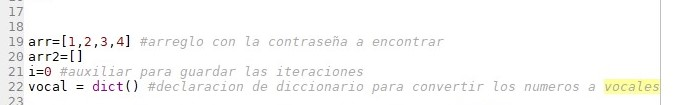
\includegraphics[scale=0.7] {img1.jpg}
\caption{Creaci\'on de arreglo.}
\label{fig:cod1}
\end{figure}

\paragraph{El siguiente paso que decid\'i hacer fue crear 4 ciclos for uno para cada car\'acter de la contrasenia, en cada uno de ellos los rangos serian de 1 a 6 ya que en total son 5 vocales.}

\paragraph{Utilice un contador para saber cuentas iteraciones fueron necesarias hasta encontrar la contrasenia, este fue introducido despu\'es del \'ultimo for. Fig: \ref{fig:cod2}}
\begin{figure}[H]
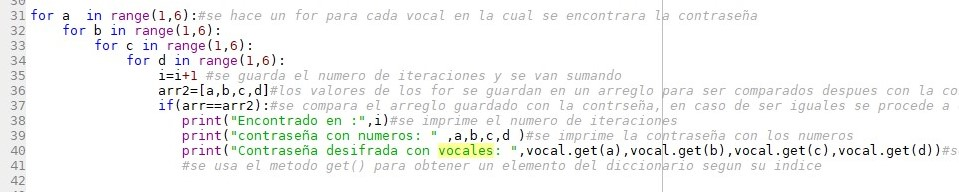
\includegraphics[scale=0.5] {img2.jpg}
\caption{Multiples for.}
\label{fig:cod2}
\end{figure}
\paragraph{Cada valor en los for fueron introducidos en un arreglo para posteriormente compararlo con el arreglo de la contrasenia por medio de un if, de no ser iguales el programa seguir\'ia comprobando car\'acter por car\'acter hasta encontrar la contrasenia, en caso de ser id\'enticos el programa imprimir\'a un mensaje con  el n\'umero de iteraci\'on y la contrasenia dada en n\'umeros donde 1=a,2=e,3=i,4=o,5=u, ya que esto no es muy practico y se necesitaba saber cual es la contrasenia en vocales, decid\'i utilizar un diccionario en los valores de las vocales esto con la finalidad de no utilizar m\'ultiples if para simplemente cambiar de n\'umeros a letras.}

 \paragraph{Para definir un nuevo diccionario utilice la funci\'on dict() y se la asigne a una variable en este caso llamada vocal.}


 
\paragraph{Una vez creado el diccionario, le asigne valores de acuerdo con la sintaxis, d\'andole a el primer elemento un valor de A, al segundo E y as\'i sucesivamente.}
\begin{figure}[H]
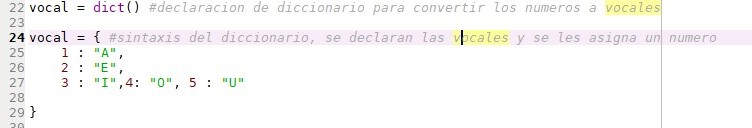
\includegraphics[scale=0.5] {img3.jpg}
\caption{Diccionario.}
\label{fig:cod3}
\end{figure}
\paragraph{Una vez hecho esto solo mande a llamar al diccionario pas\'andole la variable que conten\'ia el \'indice del for esto con el m\'etodo get() que devuelve el valor del diccionario de acuerdo al \'indice.}



\paragraph{Esto permiti\'o resolver de buena manera convertir los n\'umeros a sus respectivas vocales.}
\begin{figure}[H]
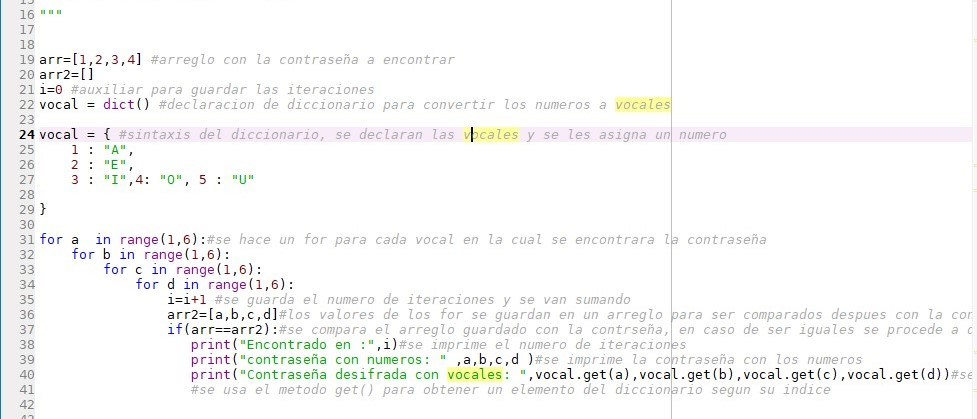
\includegraphics[scale=0.5] {img4.jpg}
\caption{Codigo Completo.}
\label{fig:cod4}
\end{figure}
\begin{figure}[H]
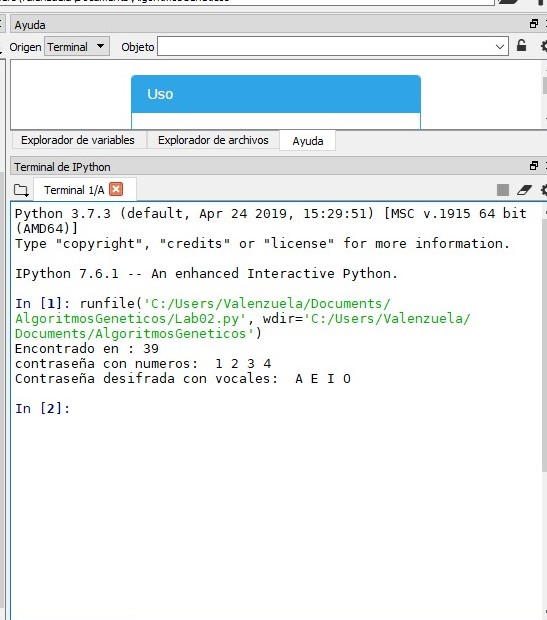
\includegraphics[scale=0.5] {img5.jpg}
\caption{Resultado.}
\label{fig:cod5}
\end{figure}
\section{Conclusi\'on}
\paragraph{En conclusi\'on, el uso de fuerza bruta para encontrar una contrasenia no es la mejor opci\'on ya que en este caso la longitud y los valores posibles en la contrasenia lo hicieron f\'acil y r\'apido de hacer, pero para contresenias mucho m\'as elaboradas y con mucho mas posibles combinaciones ser\'ia muy tardado. en este caso es de gran ayuda el uso de los algoritmos gen\'eticos para acelerar en gran medida el proceso para encontrar la contrasenia.}
\section{Referencias}
\paragraph{Montoro, A. F. (2012). Python 3 al Descubierto. RC Libros.}


\end{document}
